\FloatBarrier
\section{Administration}
\label{sec:adminPrensentation}
This section presents the administrative tool used by the administrative personnel.

The administration tool can be accessed through the site administration menu as seen in \figref{fig:navigation}.

\begin{figure}[htb]
	\centering
		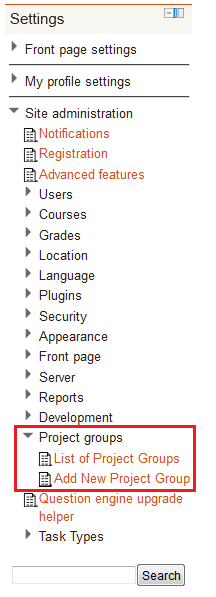
\includegraphics[scale=0.6]{images/admin-navigation.png}
	\morscaption{The settings block, which contains the site administration menu. The highlighted box displays the administrative tool for project groups} 
	\label{fig:navigation}
\end{figure}
The menu provides two links: One link to a list of all project groups, which is further described in \secref{sec:preListPg}, and another link to a page where a project group can be created, which is described in \secref{sec:addandedit}.

\FloatBarrier

\subsection{List of Project Groups}
\label{sec:preListPg}
The list of project groups, seen on \figref{fig:moodleadouplist}, provides an overview of all project groups. 
It contains a filter which can be used to reduce the number of presented project groups and thereby making it easier to find one or a set of specific project groups. 
The page contains a link to a page where project groups can be edited. 
This page is further described in \secref{sec:addandedit}.
For each project group there is a row in the list containing the following: The short name (which also works as a link to the page described in \secref{sec:projectGrpMem}), the long name of a project group, an edit button, and a delete button. 
The edit button takes the user to the same page as clicking on the ``add new project group''-link. 
The only difference is that the project group id is sent along, which forces the add \& edit page into edit mode. 

\begin{figure}
	\centering
		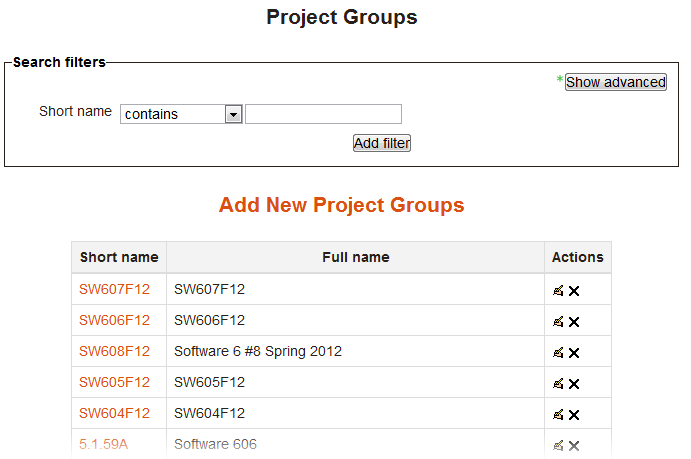
\includegraphics[width=\textwidth]{images/moodleadminprojectgrouplist.png}

	\morscaption{A screenshot of a page listing all proejct groups in the system}
		\label{fig:moodleadouplist}
\end{figure}


\FloatBarrier

\subsection{Project Group Members}
\label{sec:projectGrpMem}
%% View a group
The ``Project Group Overview'' page (seen in \figref{fig:moodlepoverview}), contains a list of the members of the project group. 
The page contains a link to the project group room (described in \secref{sec:prePgrRom}) and a link to the add \& edit page. 
For each member there is a delete button, which removes the member from the group after confirmation from the administrative user.

\begin{figure}
	\centering
		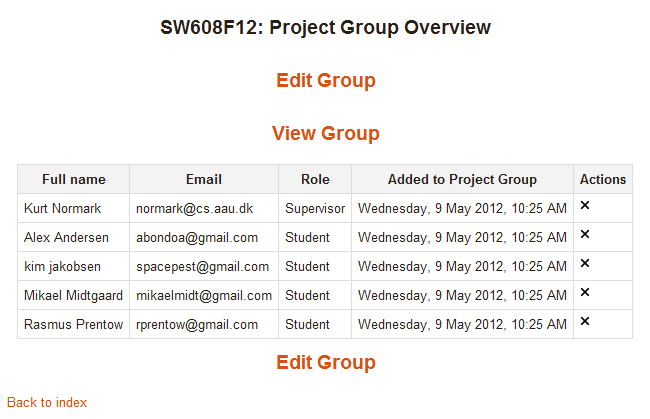
\includegraphics[width=\textwidth]{images/moodleprojectgroupoverview.png}
	\morscaption{A screenshot of the ``Project Group Overview'' page, which shows all current members of the project group}
	\label{fig:moodlepoverview}
\end{figure}
\FloatBarrier

\subsection{Add \& Edit}
\label{sec:addandedit}
%% Add/edit
The add \& edit page serves two purposes; it allows adding a project group and it allows for editing of a project group.
The page is divided into four parts and can be seen on \figref{fig:moodlcgroupedit}. 
The first part contains fields allowing the user to enter basic information of the project group which is either edited or added. 
Beneath this there is a filter.
%The filter on the add \& edit page filters users and not project groups. 
When a filter is applied the list of available users in the third part of the page is reduced according to the applied filter. 
The last part shows all added members and the user can highlight members to mark them as supervisors. 


\begin{figure}
	\centering
		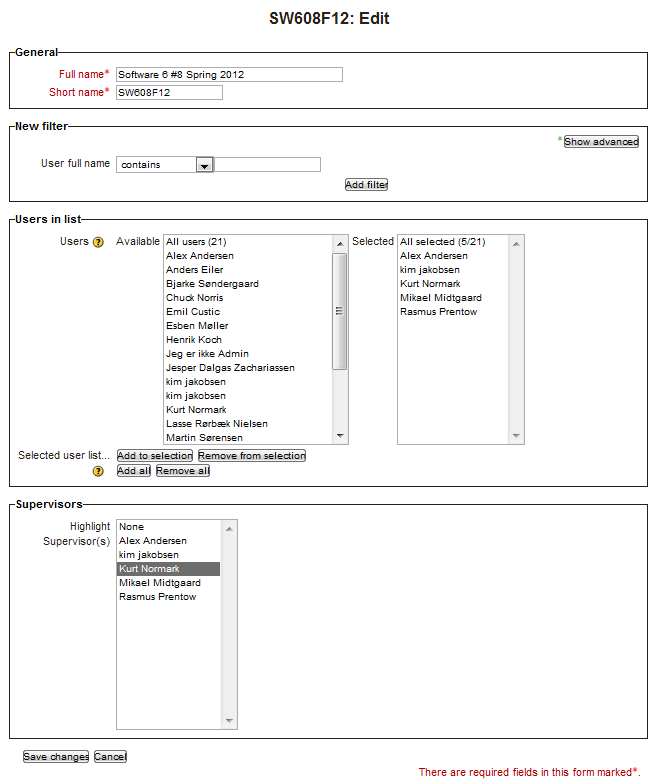
\includegraphics[width=\textwidth]{images/moodleprojecgroupedit.png}

	\morscaption{A screenshot of the add \& edit page}
		\label{fig:moodlcgroupedit}
\end{figure}
\FloatBarrier